\documentclass[11pt,a4paper]{article}
\usepackage[utf8]{inputenc}
\usepackage[margin=2cm]{geometry}
\usepackage{tikz}
\usetikzlibrary{shapes.geometric,arrows.meta,positioning,calc,fit,backgrounds,decorations.pathreplacing}
\usepackage{xcolor}
\usepackage{enumitem}
\usepackage{listings}
\usepackage{amsmath,amssymb}
\usepackage{booktabs}
\usepackage{hyperref}
\usepackage{array}

\lstset{
    language=Python,
    basicstyle=\ttfamily\scriptsize,
    keywordstyle=\color{blue}\bfseries,
    commentstyle=\color{green!50!black},
    stringstyle=\color{red!70!black},
    numbers=left,
    numberstyle=\tiny\color{gray},
    breaklines=true,
    frame=single,
    backgroundcolor=\color{gray!5},
    showstringspaces=false
}

\definecolor{inputcol}{RGB}{52,152,219}
\definecolor{embedcol}{RGB}{155,89,182}
\definecolor{slotcol}{RGB}{46,204,113}
\definecolor{crosscol}{RGB}{26,188,156}
\definecolor{selfcol}{RGB}{22,160,133}
\definecolor{lstmcol}{RGB}{241,196,15}
\definecolor{outputcol}{RGB}{231,76,60}
\definecolor{physcol}{RGB}{230,126,34}
\definecolor{metriccol}{RGB}{52,73,94}

\title{\textbf{Pile Stiffness Degradation Model (M5)}\\[0.3cm]\large 21-Slot / 21-Step Slot-Attention Transformer --- Detailed Architecture \& Code Explanation}
\author{}
\date{}

\begin{document}
\maketitle

\section{Problem}

\textbf{Goal:} Given 8 pile/soil input parameters, predict a \textbf{21-step stiffness sequence} for 3 outputs:
\begin{itemize}[nosep]
    \item $K_L$ --- lateral stiffness
    \item $K_R$ --- rotational stiffness
    \item $K_{LR}$ --- cross-coupling stiffness
\end{itemize}

The M5 project keeps the same overall architecture philosophy as M4.1, but it changes the temporal target structure:
\begin{itemize}[nosep]
    \item M4.1 predicted 44 steps.
    \item M5 predicts 21 steps.
    \item Slot 1 predicts the \textbf{initial absolute stiffness values}.
    \item The remaining 20 slots are used to generate the \textbf{ordered sequential drops} that build the rest of the curve.
\end{itemize}

The final sequence is cumulative: later steps depend on earlier predicted drops, so the model cannot reach step $t$ without first constructing all previous steps.

\section{What Makes M5 Different from M4.1}

The main conceptual difference is not the low-level neural modules, but \textbf{how the time axis is represented and interpreted}.

\subsection*{Difference 1: 21 prediction steps instead of 44}
The original Excel data still stores 44 points per scenario, but M5 reduces them to 21 representative positions using:

$$
\texttt{STEP\_INDICES} = [0, 2, 4, 6, 9, 11, 13, 15, 17, 19, 22, 24, 26, 28, 30, 32, 34, 37, 39, 41, 43]
$$

So M5 does not invent a new raw dataset. It \textbf{subsamples the original 44-step physical sequence} into 21 ordered states.

\subsection*{Difference 2: Slot interpretation is now aligned with the 21-step target}
The model still has 21 slots, but their meaning is now easier to align with the target:

\begin{itemize}[nosep]
    \item \textbf{Slot 1} represents the initial state and predicts step 1 directly.
    \item \textbf{Slots 2--21} represent the information needed to build the remaining 20 transitions.
\end{itemize}

Important implementation detail: the code does \textbf{not} force each drop slot to map one-to-one to one exact decoder step with a hard wiring. Instead, the 20 drop slots are:
\begin{itemize}[nosep]
    \item averaged to form the repeated decoder input,
    \item then reused through decoder cross-attention so each decoded step can attend to the 20 drop slots.
\end{itemize}

So conceptually the architecture is ``slot 1 = initial, other slots = ordered degradation information'', while operationally the LSTM + cross-attention decides how to use those drop slots across the 20 remaining steps.

\subsection*{Difference 3: The M5 web application is much richer}
M4.1 mainly visualized target vs predicted curves. M5 still does that, but also computes and displays:

\begin{itemize}[nosep]
    \item overall system accuracy,
    \item per-variable accuracy for $K_L$, $K_R$, $K_{LR}$,
    \item per-slot accuracy,
    \item per-scenario accuracy,
    \item per-step target vs predicted tables.
\end{itemize}

The metrics used are:
\begin{itemize}[nosep]
    \item \textbf{$R^2$}: Coefficient of Determination
    \item \textbf{RMSE}: Root Mean Squared Error
    \item \textbf{MAE}: Mean Absolute Error
\end{itemize}

\section{Inputs and Outputs}

\subsection*{Input features}
Each scenario is represented by 8 scalar inputs:

\begin{enumerate}[nosep]
    \item PI
    \item $G_{max}$
    \item $\nu$
    \item $D_p$
    \item $T_p$
    \item $L_p$
    \item $I_p$
    \item $D_p/L_p$
\end{enumerate}

The input tensor shape is:
$$
[B, 8]
$$

\subsection*{Output sequence}
For each scenario, the model predicts 21 states, and each state contains 3 values:

$$
[B, 21, 3]
$$

where the 3 channels are:
$$
[K_L, K_R, K_{LR}]
$$

The sequence semantics are:
\begin{itemize}[nosep]
    \item Step 1: initial absolute stiffness values.
    \item Steps 2--21: values obtained after cumulative application of predicted drops.
\end{itemize}

\section{Data Pipeline}

\subsection*{Raw Excel format}
The source file is \texttt{REAL DATA.xlsx}. Each physical scenario appears as 44 rows:
\begin{itemize}[nosep]
    \item row 1 of the group = initial absolute values,
    \item rows 2--44 = drops between successive states.
\end{itemize}

So the raw table stores a mixture of:
\begin{itemize}[nosep]
    \item one absolute starting point,
    \item then a list of incremental degradations.
\end{itemize}

\subsection*{Reconstruction of the 44 absolute values}
The code first reconstructs the 44-state absolute sequence:

$$
K(1) = K^0
$$

$$
K(t) = K^0 - \sum_{n=1}^{t-1} \text{drop}_n \qquad t=2,\dots,44
$$

In code terms:
\begin{itemize}[nosep]
    \item read the first row as \texttt{initial},
    \item read the next 43 rows as \texttt{drops},
    \item compute cumulative sum of drops,
    \item subtract cumulative drops from the initial value.
\end{itemize}

\subsection*{Subsampling from 44 steps to 21 steps}
After reconstructing the full 44-state sequence, M5 selects only the following positions:

\begin{center}
\begin{tabular}{>{\ttfamily}c c}
\toprule
21-step position & Original 44-step index \\
\midrule
1 & 0 \\
2 & 2 \\
3 & 4 \\
4 & 6 \\
5 & 9 \\
6 & 11 \\
7 & 13 \\
8 & 15 \\
9 & 17 \\
10 & 19 \\
11 & 22 \\
12 & 24 \\
13 & 26 \\
14 & 28 \\
15 & 30 \\
16 & 32 \\
17 & 34 \\
18 & 37 \\
19 & 39 \\
20 & 41 \\
21 & 43 \\
\bottomrule
\end{tabular}
\end{center}

This is a deterministic downsampling strategy. It keeps the beginning, middle, and end of the degradation path while reducing the temporal length that the network must predict.

\subsection*{Scaling strategy}
M5 uses the same robust scaling philosophy as M4.1:

\begin{itemize}[nosep]
    \item Inputs are scaled with \texttt{RobustScaler}.
    \item Outputs are transformed using:
    $$
    y_{\log} = \mathrm{sign}(y) \cdot \log(1 + |y|)
    $$
    \item Then the transformed outputs are also scaled with \texttt{RobustScaler}.
\end{itemize}

This is important because stiffness values can span very different magnitudes, especially $K_R$ which is much larger than $K_L$.

\subsection*{Train/test split}
The code uses:
\begin{itemize}[nosep]
    \item 80\% training,
    \item 20\% testing,
    \item \texttt{random\_state=42} for reproducibility.
\end{itemize}

With the current data used in M5:
\begin{itemize}[nosep]
    \item total scenarios: 1019,
    \item training scenarios: 815,
    \item test scenarios: 204.
\end{itemize}

\section{Complete Model Architecture}

The model has 5 major stages:

\begin{enumerate}[nosep]
    \item Input embedding
    \item Iterative slot refinement
    \item Slot split into initial branch and drop branch
    \item Sequential decoding of 20 post-initial states
    \item Cumulative sequence assembly
\end{enumerate}

\subsection*{Stage 1: Input embedding}
The 8 input scalars are projected into a 64-dimensional latent vector using:
\begin{itemize}[nosep]
    \item \texttt{Linear(8, 64)}
    \item \texttt{LayerNorm(64)}
    \item \texttt{GELU}
\end{itemize}

This produces a tensor of shape:
$$
[B, 1, 64]
$$

So the whole scenario is encoded as one compact latent token.

\subsection*{Stage 2: Learnable slot bank}
The model contains 21 learnable slot vectors:

$$
\texttt{slots} \in \mathbb{R}^{1 \times 21 \times 64}
$$

During the forward pass, these are expanded over the batch dimension:
$$
[B, 21, 64]
$$

Their intended roles are:
\begin{itemize}[nosep]
    \item Slot 1: initial state descriptor
    \item Slots 2--21: degradation descriptors
\end{itemize}

\subsection*{Stage 3: Slot refinement loop}
The slots are refined over 2 iterations. Each iteration contains 3 sub-operations:

\subsubsection*{3.1 Cross-attention}
Each slot attends to the embedded input token.

Operationally:
\begin{itemize}[nosep]
    \item Query = slots
    \item Key = input embedding
    \item Value = input embedding
\end{itemize}

So each slot updates itself based on the single scenario representation.

\subsubsection*{3.2 Self-attention}
The refined slots then attend to each other. This allows slot coordination and avoids all slots learning the exact same feature.

Operationally:
\begin{itemize}[nosep]
    \item Query = slots
    \item Key = slots
    \item Value = slots
\end{itemize}

\subsubsection*{3.3 Per-slot MLP}
Each slot passes through a feedforward block:

$$
64 \rightarrow 128 \rightarrow 64
$$

with GELU and dropout.

Every sub-block uses residual addition plus layer normalization.

\subsection*{Stage 4: Slot split}
After refinement, the 21 slots are divided into two branches.

\subsubsection*{Branch A: Slot 1}
Slot 1 is used in two ways:

\begin{enumerate}[nosep]
    \item It is passed through the \textbf{initial head} to predict the first absolute stiffness vector:
    $$
    [K_L^0, K_R^0, K_{LR}^0]
    $$
    \item It is projected into the initial hidden state $h_0$ and cell state $c_0$ of the LSTM.
\end{enumerate}

The initial head is:
$$
64 \rightarrow 32 \rightarrow 3
$$

The LSTM state projections are:
$$
h_0: 64 \rightarrow 128
$$
$$
c_0: 64 \rightarrow 128
$$

These 128 values are reshaped into:
$$
[2, B, 64]
$$

because the decoder LSTM has 2 layers and hidden size 64.

\subsubsection*{Branch B: Slots 2--21}
The 20 remaining slots are used as the degradation memory. In the current implementation they are used in two ways:

\begin{enumerate}[nosep]
    \item Mean pooling over the 20 slots to create a shared decoder input template.
    \item Direct reuse as keys/values in decoder cross-attention.
\end{enumerate}

\subsection*{Stage 5: Decoder input construction}
The mean of Slots 2--21 has shape:
$$
[B, 1, 64]
$$

This vector is repeated 20 times because M5 must predict 20 post-initial states:
$$
[B, 20, 64]
$$

Then a learned positional embedding is added:
$$
\texttt{pos\_embed} \in \mathbb{R}^{1 \times 21 \times 64}
$$

Only the first 20 positions after step 1 are used in decoder input construction:
$$
\texttt{pos\_embed[:, :seq\_len-1, :]}
$$

This provides step identity so the decoder can distinguish early drops from late drops.

\subsection*{Stage 6: LSTM decoder}
The decoder is a 2-layer LSTM with hidden size 64.

Input shape:
$$
[B, 20, 64]
$$

Initial state:
$$
h_0, c_0 \in \mathbb{R}^{2 \times B \times 64}
$$

Output shape:
$$
[B, 20, 64]
$$

Its job is to model the ordered temporal progression of degradation.

\subsection*{Stage 7: Decoder cross-attention}
Each of the 20 decoder states attends back to the 20 degradation slots:

\begin{itemize}[nosep]
    \item Query = LSTM outputs
    \item Key = Slots 2--21
    \item Value = Slots 2--21
\end{itemize}

This lets each time step select the slot information most relevant to that step.

Again, residual addition plus layer normalization are applied.

\subsection*{Stage 8: Drop projection and physics constraints}
The decoder output is mapped to 3 drop values per step through:

$$
64 \rightarrow 32 \rightarrow 3
$$

Then the following physical rule is enforced:

\begin{itemize}[nosep]
    \item $K_L$ drop is forced non-positive
    \item $K_R$ drop is forced non-positive
    \item $K_{LR}$ drop is left unconstrained
\end{itemize}

In code:
\begin{align*}
\Delta K_L &= -|\hat{d}_1| \\
\Delta K_R &= -|\hat{d}_2| \\
\Delta K_{LR} &= \hat{d}_3
\end{align*}

This means the model is not allowed to create positive increments for $K_L$ and $K_R$.

\subsection*{Stage 9: Cumulative output assembly}
The 20 decoded drops are accumulated:

$$
\text{cumulative}(t) = \sum_{n=1}^{t} d_n
$$

Then added to the initial prediction:

$$
K(t) = K^0 + \sum_{n=1}^{t-1} d_n
$$

So the final output is:
\begin{itemize}[nosep]
    \item one initial state from Slot 1,
    \item plus 20 subsequent states built from cumulative drops.
\end{itemize}

Final shape:
$$
[B, 21, 3]
$$

\section{Detailed Architecture Diagram}

\begin{center}
\resizebox{\textwidth}{!}{%
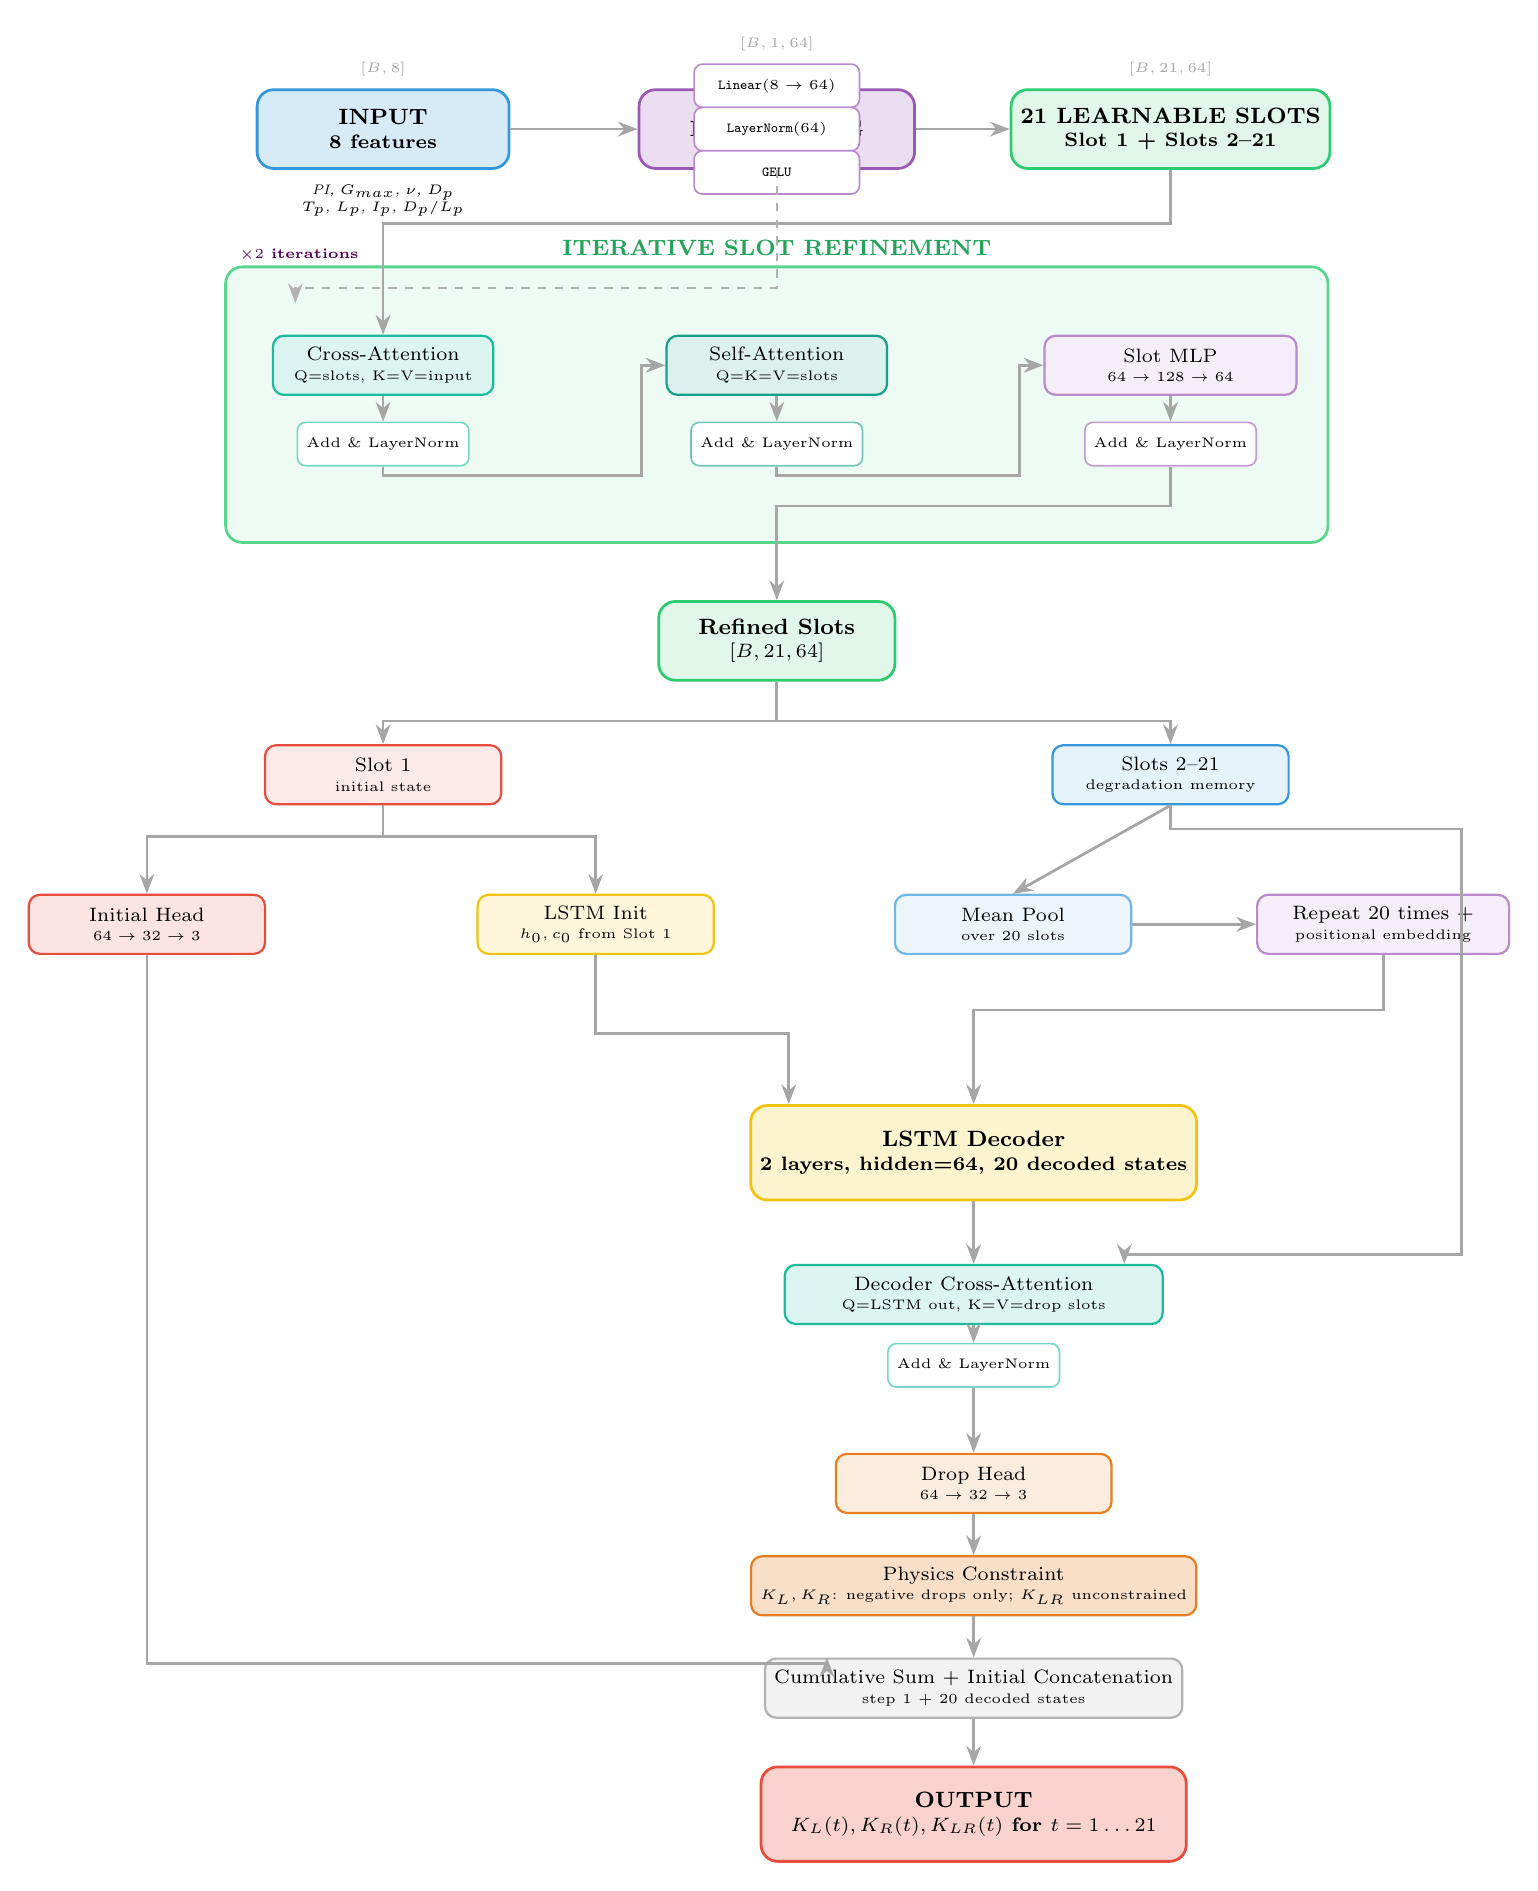
\begin{tikzpicture}[
    >={Stealth[length=2.5mm]},
    block/.style={rectangle, rounded corners=6pt, minimum width=3.2cm, minimum height=1cm, align=center, font=\footnotesize\bfseries, draw, line width=1pt},
    smallblock/.style={rectangle, rounded corners=4pt, minimum width=2.8cm, minimum height=0.75cm, align=center, font=\scriptsize, draw, line width=0.8pt},
    tinyblock/.style={rectangle, rounded corners=3pt, minimum width=2.1cm, minimum height=0.55cm, align=center, font=\tiny, draw, line width=0.6pt},
    arrow/.style={->, thick, gray!70, line width=1pt},
    dashedarrow/.style={->, dashed, gray!60, line width=0.8pt},
    note/.style={font=\tiny\itshape, align=center, text width=2.6cm},
    dimlab/.style={font=\tiny\ttfamily, text=gray!70},
    looplab/.style={font=\tiny\bfseries, text=violet!70!black},
]

\node[block, fill=inputcol!20, draw=inputcol] (inp) at (0,0)
    {INPUT\\[-1pt]{\scriptsize 8 features}};
\node[note, below=2pt of inp] {PI, $G_{max}$, $\nu$, $D_p$\\$T_p$, $L_p$, $I_p$, $D_p/L_p$};
\node[dimlab, above=1pt of inp] {$[B, 8]$};

\node[block, fill=embedcol!20, draw=embedcol, minimum width=3.5cm] (emb) at (5,0)
    {EMBEDDING};
\node[tinyblock, fill=white, draw=embedcol!70] (emb1) at (5, 0.55) {\texttt{Linear}$(8 \to 64)$};
\node[tinyblock, fill=white, draw=embedcol!70] (emb2) at (5, 0) {\texttt{LayerNorm}$(64)$};
\node[tinyblock, fill=white, draw=embedcol!70] (emb3) at (5, -0.55) {\texttt{GELU}};
\node[dimlab, above=1pt of emb1] {$[B, 1, 64]$};

\node[block, fill=slotcol!15, draw=slotcol, minimum width=3.8cm] (slotinit) at (10,0)
    {21 LEARNABLE SLOTS\\[-1pt]{\scriptsize Slot 1 + Slots 2--21}};
\node[dimlab, above=1pt of slotinit] {$[B, 21, 64]$};

\draw[arrow] (inp) -- (emb);
\draw[arrow] (emb) -- (slotinit);

\node[block, fill=slotcol!8, draw=slotcol!80, minimum width=14cm, minimum height=3.5cm]
    (refine_box) at (5, -3.5) {};
\node[above=0pt of refine_box.north, font=\footnotesize\bfseries, slotcol!80!black]
    {ITERATIVE SLOT REFINEMENT};
\node[looplab, above right=-2pt and 2pt of refine_box.north west]
    {$\times 2$ iterations};

\node[smallblock, fill=crosscol!15, draw=crosscol] (crossattn) at (0, -3)
    {Cross-Attention\\[-1pt]{\tiny Q=slots, K=V=input}};
\node[tinyblock, fill=white, draw=crosscol!60] (crossnorm) at (0, -4)
    {Add \& LayerNorm};

\node[smallblock, fill=selfcol!15, draw=selfcol] (selfattn) at (5, -3)
    {Self-Attention\\[-1pt]{\tiny Q=K=V=slots}};
\node[tinyblock, fill=white, draw=selfcol!60] (selfnorm) at (5, -4)
    {Add \& LayerNorm};

\node[smallblock, fill=embedcol!10, draw=embedcol!70, minimum width=3.2cm] (mlp) at (10, -3)
    {Slot MLP\\[-1pt]{\tiny $64 \to 128 \to 64$}};
\node[tinyblock, fill=white, draw=embedcol!60] (mlpnorm) at (10, -4)
    {Add \& LayerNorm};

\draw[arrow] (crossattn) -- (crossnorm);
\draw[arrow] (crossnorm) -- ++(0,-0.4) -| ($(selfattn.south west)-(0.3,0)$) |- (selfattn.west);
\draw[arrow] (selfattn) -- (selfnorm);
\draw[arrow] (selfnorm) -- ++(0,-0.4) -| ($(mlp.south west)-(0.3,0)$) |- (mlp.west);
\draw[arrow] (mlp) -- (mlpnorm);

\draw[arrow] (slotinit) -- ++(0,-1.2) -| (crossattn.north);
\draw[dashedarrow] (emb.south) -- ++(0,-1.5) -| ($(crossattn.north west)+(0.3,0.4)$);

\node[block, fill=slotcol!15, draw=slotcol, minimum width=3cm] (refined) at (5, -6.5)
    {Refined Slots\\[-1pt]{\scriptsize $[B, 21, 64]$}};
\draw[arrow] (mlpnorm.south) -- ++(0,-0.5) -| (refined.north);

\node[smallblock, fill=outputcol!12, draw=outputcol, minimum width=3cm] (slot1) at (0, -8.2)
    {Slot 1\\[-1pt]{\tiny initial state}};
\node[smallblock, fill=inputcol!12, draw=inputcol, minimum width=3cm] (slots220) at (10, -8.2)
    {Slots 2--21\\[-1pt]{\tiny degradation memory}};

\draw[arrow] (refined.south) -- ++(0,-0.5) -| (slot1.north);
\draw[arrow] (refined.south) -- ++(0,-0.5) -| (slots220.north);

\node[smallblock, fill=outputcol!15, draw=outputcol, minimum width=3cm] (inithead) at (-3, -10.1)
    {Initial Head\\[-1pt]{\tiny $64 \to 32 \to 3$}};
\node[smallblock, fill=lstmcol!15, draw=lstmcol, minimum width=3cm] (h0c0) at (2.7, -10.1)
    {LSTM Init\\[-1pt]{\tiny $h_0,c_0$ from Slot 1}};
\node[smallblock, fill=inputcol!10, draw=inputcol!70, minimum width=3cm] (meanagg) at (8.0, -10.1)
    {Mean Pool\\[-1pt]{\tiny over 20 slots}};
\node[smallblock, fill=embedcol!10, draw=embedcol!70, minimum width=3.2cm] (posemb) at (12.7, -10.1)
    {Repeat 20 times +\\[-1pt]{\tiny positional embedding}};

\draw[arrow] (slot1.south) -- ++(0,-0.4) -| (inithead.north);
\draw[arrow] (slot1.south) -- ++(0,-0.4) -| (h0c0.north);
\draw[arrow] (slots220.south) -- (meanagg.north);
\draw[arrow] (meanagg) -- (posemb);

\node[block, fill=lstmcol!20, draw=lstmcol, minimum width=4.8cm, minimum height=1.2cm] (lstm) at (7.5, -13)
    {LSTM Decoder\\[-1pt]{\scriptsize 2 layers, hidden=64, 20 decoded states}};
\draw[arrow] (posemb.south) -- ++(0,-0.7) -| (lstm.north);
\draw[arrow] (h0c0.south) -- ++(0,-1.0) -| ($(lstm.north west)+(0.5,0)$);

\node[smallblock, fill=crosscol!15, draw=crosscol, minimum width=4.8cm] (deccross) at (7.5, -14.8)
    {Decoder Cross-Attention\\[-1pt]{\tiny Q=LSTM out, K=V=drop slots}};
\node[tinyblock, fill=white, draw=crosscol!60] (decnorm) at (7.5, -15.7)
    {Add \& LayerNorm};

\draw[arrow] (lstm) -- (deccross);
\draw[arrow] (deccross) -- (decnorm);
\draw[arrow] (slots220.south) -- ++(0,-0.3) -- ++(3.7,0) -- ++(0,-5.4) -| ($(deccross.north east)-(0.5,0)$);

\node[smallblock, fill=physcol!15, draw=physcol, minimum width=3.5cm] (drophead) at (7.5, -17.2)
    {Drop Head\\[-1pt]{\tiny $64 \to 32 \to 3$}};
\node[smallblock, fill=physcol!25, draw=physcol, minimum width=5.6cm] (physics) at (7.5, -18.5)
    {Physics Constraint\\[-1pt]{\tiny $K_L,K_R$: negative drops only; $K_{LR}$ unconstrained}};
\node[smallblock, fill=gray!10, draw=gray!60, minimum width=4.6cm] (cumsum) at (7.5, -19.8)
    {Cumulative Sum + Initial Concatenation\\[-1pt]{\tiny step 1 + 20 decoded states}};
\node[block, fill=outputcol!25, draw=outputcol, minimum width=5.4cm, minimum height=1.2cm] (output) at (7.5, -21.4)
    {OUTPUT\\[-1pt]{\scriptsize $K_L(t), K_R(t), K_{LR}(t)$ for $t=1\ldots21$}};

\draw[arrow] (decnorm) -- (drophead);
\draw[arrow] (drophead) -- (physics);
\draw[arrow] (physics) -- (cumsum);
\draw[arrow] (cumsum) -- (output);
\draw[arrow] (inithead.south) -- ++(0,-9.0) -| ($(cumsum.north west)+(0.8,0)$);

\end{tikzpicture}
}%
\end{center}

\section{Forward Pass Explained Step by Step}

The forward pass implements the architecture exactly as follows:

\begin{enumerate}[nosep]
    \item Embed the 8 inputs into one 64-dimensional token.
    \item Expand the 21 learnable slots over the batch.
    \item Run 2 refinement rounds: cross-attention, self-attention, MLP.
    \item Split slots into Slot 1 and Slots 2--21.
    \item Decode the initial stiffness vector from Slot 1.
    \item Convert Slot 1 into $h_0$ and $c_0$ for the LSTM.
    \item Mean-pool the 20 drop slots, repeat them for 20 steps, add positional embeddings.
    \item Run the 2-layer LSTM over these 20 decoder inputs.
    \item Refine the LSTM outputs with decoder cross-attention to the 20 drop slots.
    \item Project refined decoder states to 3 drops.
    \item Enforce sign constraints on $K_L$ and $K_R$ drops.
    \item Apply cumulative sum and prepend the initial prediction.
\end{enumerate}

\begin{lstlisting}
def forward(self, x, seq_len=None):
    if seq_len is None:
        seq_len = self.max_seq_len
    batch_size = x.size(0)

    # 1) Embed input
    x_embed = self.input_embed(x).unsqueeze(1)      # [B, 1, 64]

    # 2) Expand slots
    slots = self.slots.expand(batch_size, -1, -1)   # [B, 21, 64]

    # 3) Two refinement rounds
    for _ in range(self.num_iterations):
        cross_out, _ = self.cross_attn(slots, x_embed, x_embed)
        slots = self.cross_norm(slots + cross_out)
        self_out, _ = self.self_attn(slots, slots, slots)
        slots = self.self_norm(slots + self_out)
        slots = self.mlp_norm(slots + self.slot_mlp(slots))

    # 4) Split slots
    slot_initial = slots[:, 0:1, :]
    slot_drops = slots[:, 1:, :]

    # 5) Initial absolute prediction
    initial_decoded = self.initial_proj(slot_initial)  # [B, 1, 3]

    # 6) LSTM initial state from Slot 1
    init_vec = slot_initial.squeeze(1)
    h0 = self.h0_proj(init_vec).view(batch_size, 2, self.d_model)
    h0 = h0.permute(1, 0, 2).contiguous()
    c0 = self.c0_proj(init_vec).view(batch_size, 2, self.d_model)
    c0 = c0.permute(1, 0, 2).contiguous()

    # 7) Decoder input from mean-pooled drop slots + position
    drop_agg = slot_drops.mean(dim=1, keepdim=True)
    drop_agg = drop_agg.expand(-1, seq_len - 1, -1)
    decoder_input = drop_agg + self.pos_embed[:, :seq_len - 1, :]

    # 8) Sequential decoding
    lstm_out, _ = self.seq_decoder(decoder_input, (h0, c0))

    # 9) Cross-attention back to drop slots
    refined = self.decoder_cross_attn(lstm_out, slot_drops, slot_drops)[0]
    refined = self.decoder_cross_norm(lstm_out + refined)

    # 10) Project to drops
    raw_drops = self.drop_proj(refined)

    # 11) Physics constraints
    drops_kl_kr = -torch.abs(raw_drops[:, :, :2])
    drops_klr = raw_drops[:, :, 2:3]
    drops = torch.cat([drops_kl_kr, drops_klr], dim=2)

    # 12) Build final sequence
    cumulative_drops = torch.cumsum(drops, dim=1)
    stiffness_after_drops = initial_decoded + cumulative_drops
    stiffness_seq = torch.cat([initial_decoded, stiffness_after_drops], dim=1)
    return stiffness_seq
\end{lstlisting}

\section{Model Definition Code Explained}

\subsection*{Embedding block}
This turns the 8 raw input values into a learned hidden representation.

\begin{lstlisting}
self.input_embed = nn.Sequential(
    nn.Linear(input_size, d_model),
    nn.LayerNorm(d_model),
    nn.GELU(),
)
\end{lstlisting}

\subsection*{Learnable slots}
These are trainable vectors that specialize during training.

\begin{lstlisting}
self.slots = nn.Parameter(torch.randn(1, num_slots, d_model) * 0.02)
\end{lstlisting}

\subsection*{Refinement layers}
These modules implement the iterative slot update mechanism.

\begin{lstlisting}
self.cross_attn = nn.MultiheadAttention(d_model, num_heads,
                                        dropout=dropout,
                                        batch_first=True)
self.cross_norm = nn.LayerNorm(d_model)

self.self_attn = nn.MultiheadAttention(d_model, num_heads,
                                       dropout=dropout,
                                       batch_first=True)
self.self_norm = nn.LayerNorm(d_model)

self.slot_mlp = nn.Sequential(
    nn.Linear(d_model, d_model * 2),
    nn.GELU(),
    nn.Dropout(dropout),
    nn.Linear(d_model * 2, d_model),
)
self.mlp_norm = nn.LayerNorm(d_model)
\end{lstlisting}

\subsection*{Initial-value branch}
This branch produces the first absolute state and initializes the recurrent decoder.

\begin{lstlisting}
self.h0_proj = nn.Linear(d_model, d_model * 2)
self.c0_proj = nn.Linear(d_model, d_model * 2)

self.initial_proj = nn.Sequential(
    nn.Linear(d_model, d_model // 2),
    nn.GELU(),
    nn.Linear(d_model // 2, 3),
)
\end{lstlisting}

\subsection*{Sequential decoder branch}
This branch produces the 20 post-initial states.

\begin{lstlisting}
self.seq_decoder = nn.LSTM(d_model, d_model, 2,
                           batch_first=True, dropout=dropout)

self.decoder_cross_attn = nn.MultiheadAttention(
    d_model, num_heads, dropout=dropout, batch_first=True)
self.decoder_cross_norm = nn.LayerNorm(d_model)

self.drop_proj = nn.Sequential(
    nn.Linear(d_model, d_model // 2),
    nn.GELU(),
    nn.Linear(d_model // 2, 3),
)

self.pos_embed = nn.Parameter(torch.randn(1, max_seq_len, d_model) * 0.02)
\end{lstlisting}

\section{Training Logic}

\subsection*{Loss design}
The training script uses a 3-part composite loss:

\begin{enumerate}[nosep]
    \item \textbf{Sequence loss} --- Huber loss on all predicted values.
    \item \textbf{Initial loss} --- MSE on the first state only, multiplied by 3.
    \item \textbf{Shape loss} --- Huber loss on first differences between successive steps.
\end{enumerate}

This is important because M5 must simultaneously:
\begin{itemize}[nosep]
    \item get the absolute starting point correct,
    \item keep the whole sequence close to the target,
    \item preserve the degradation shape from one step to the next.
\end{itemize}

\begin{lstlisting}
loss_seq = huber(pred, Y_batch)
loss_initial = mse(pred[:, 0, :], Y_batch[:, 0, :]) * 3.0

diff_pred = pred[:, 1:, :] - pred[:, :-1, :]
diff_target = Y_batch[:, 1:, :] - Y_batch[:, :-1, :]
loss_shape = huber(diff_pred, diff_target)

loss = loss_seq + loss_initial + loss_shape
\end{lstlisting}

\subsection*{Optimization settings}
\begin{itemize}[nosep]
    \item Optimizer: AdamW
    \item Learning rate: 0.0005
    \item Weight decay: 0.01
    \item Batch size: 4
    \item Maximum epochs: 3000
    \item Scheduler: ReduceLROnPlateau with patience 100, factor 0.5
    \item Early stopping patience: 300
\end{itemize}

Gradients are clipped to norm 1.0 to stabilize training.

\subsection*{Actual training outcome in M5}
Training stopped early at epoch 928.

The script reported the following final metrics on the test set (original scale):

\begin{center}
\begin{tabular}{@{}lccc@{}}
\toprule
Metric target & $R^2$ & RMSE & MAE \\
\midrule
Overall & 0.9913 & 1.9776e+10 & 2.9776e+09 \\
$K_L$ & 0.9907 & 6.2096e+07 & 2.1091e+07 \\
$K_R$ & 0.9838 & 3.4232e+10 & 8.5620e+09 \\
$K_{LR}$ & 0.9882 & 1.1838e+09 & 3.4965e+08 \\
\bottomrule
\end{tabular}
\end{center}

These results show that the 21-step M5 formulation still preserves very high predictive accuracy.

\section{Per-Slot Interpretation}

The model also evaluates each slot position separately after sequence reconstruction. In the saved metrics:

\begin{itemize}[nosep]
    \item Slot 1 corresponds to the initial absolute state.
    \item Slots 2--21 correspond to the successive degradation states after cumulative drop application.
\end{itemize}

The per-slot overall $R^2$ values improved from early to late steps and were approximately in this range:
\begin{itemize}[nosep]
    \item Slot 1: 0.9908
    \item Slot 10: 0.9902
    \item Slot 15: 0.9927
    \item Slot 21: 0.9968
\end{itemize}

This means the model remained accurate across the full predicted sequence and became even more accurate on later states for this test split.

\section{Web Application Architecture}

The M5 web application is not just a plotting tool. It is a second inference and reporting layer built on top of the saved training artifacts.

\subsection*{Artifacts loaded by the web app}
At startup, the web app loads:

\begin{itemize}[nosep]
    \item \texttt{scaler\_X.pkl}
    \item \texttt{scaler\_y.pkl}
    \item \texttt{feature\_names.pkl}
    \item \texttt{max\_seq\_len.pkl}
    \item \texttt{test\_data.pkl}
    \item \texttt{pile\_model.pth}
\end{itemize}

Then it reconstructs the model, reruns prediction on the stored test set, inverses the scaling, and computes metrics for display.

\subsection*{Accuracy layers shown in the UI}
The web app computes and displays four nested levels of accuracy:

\begin{enumerate}[nosep]
    \item \textbf{Overall system metrics}
    \item \textbf{Per-variable metrics}
    \item \textbf{Per-slot metrics}
    \item \textbf{Per-scenario metrics}
\end{enumerate}

\subsection*{Frontend layout}
The browser UI contains:

\begin{itemize}[nosep]
    \item a top banner with overall $R^2$, RMSE, MAE,
    \item 3 variable cards for $K_L$, $K_R$, $K_{LR}$,
    \item a list of test scenarios,
    \item a scenario detail panel,
    \item 3 line charts comparing target vs predicted values,
    \item a per-step table with percentage errors,
    \item a bottom per-slot accuracy table.
\end{itemize}

\subsection*{Metric computation code}
The metric helper used in both training and the web app is:

\begin{lstlisting}
def calc_metrics(y_true, y_pred):
    ft, fp = y_true.flatten(), y_pred.flatten()
    return {
        'r2': float(r2_score(ft, fp)),
        'rmse': float(np.sqrt(mean_squared_error(ft, fp))),
        'mae': float(mean_absolute_error(ft, fp)),
    }
\end{lstlisting}

\subsection*{Scenario table semantics}
For each scenario, the UI shows:
\begin{itemize}[nosep]
    \item raw input parameters,
    \item scenario-level $R^2$, RMSE, MAE,
    \item per-variable scenario metrics,
    \item step-by-step target and predicted values,
    \item error percentage for every output at every step.
\end{itemize}

So the web app is designed not only to demonstrate predictions, but also to inspect where and how prediction error is distributed.

\section{Saved Files Produced by Training}

After running \texttt{train.py}, the M5 folder stores:

\begin{center}
\begin{tabular}{@{}ll@{}}
\toprule
File & Purpose \\
\midrule
\texttt{pile\_model.pth} & trained model weights \\
\texttt{scaler\_X.pkl} & input scaler \\
\texttt{scaler\_y.pkl} & output scaler \\
\texttt{feature\_names.pkl} & ordered input feature names \\
\texttt{max\_seq\_len.pkl} & stored sequence length (=21) \\
\texttt{test\_data.pkl} & held-out test set for the web app \\
\texttt{model\_metrics.pkl} & saved overall/per-variable/per-slot metrics \\
\bottomrule
\end{tabular}
\end{center}

\section{Code Summary}

The whole M5 project can be understood as the following pipeline:

\begin{enumerate}[nosep]
    \item Read 44-row scenarios from Excel.
    \item Reconstruct absolute 44-step stiffness curves from initial values and drops.
    \item Downsample each curve to 21 representative states.
    \item Scale inputs and transformed outputs.
    \item Encode the scenario into 21 learnable slots.
    \item Use Slot 1 for the initial state and LSTM initialization.
    \item Use Slots 2--21 as degradation memory for sequential decoding.
    \item Predict 20 ordered drops, apply cumulative reconstruction, and obtain a 21-step sequence.
    \item Evaluate accuracy globally, per variable, per slot, and per scenario.
    \item Serve an interactive web interface for analysis and visualization.
\end{enumerate}

\section{How to Use}

\begin{enumerate}[nosep]
    \item Run \texttt{python train.py} to train the model and save all artifacts.
    \item Run \texttt{python webapp.py} to start the Flask server.
    \item Open \texttt{http://127.0.0.1:5000} in the browser.
    \item Explore overall metrics, variable metrics, slot metrics, and scenario-by-scenario predictions.
\end{enumerate}

\end{document}